\documentclass[10pt]{beamer}

% Tema Limpo e Profissional (Padrao Institucional IFCE Taua)
\usetheme{Madrid}
\usecolortheme{whale}

% Pacotes Essenciais
\usepackage[utf8]{inputenc}
\usepackage[T1]{fontenc}
\usepackage[portuguese]{babel}
\usepackage{graphicx}
\usepackage{booktabs}
\usepackage{amsmath}
\usepackage{amssymb}
\usepackage{listings}
\usepackage{xcolor}

% Configuracoes de Codigo (Python)
\lstset{
    language=Python,
    basicstyle=\ttfamily\scriptsize,
    keywordstyle=\color{blue}\bfseries,
    stringstyle=\color{red!80!black},
    commentstyle=\color{green!60!black},
    breaklines=true,
    showstringspaces=false,
    tabsize=4
}

% Metadados da Apresentacao
\title[IFCE Tauá - Engenharia de Software]{Aula 22: Diagramas de Interação e Máquina de Estados}
\subtitle{Fundamentação Comportamental baseada nos Capítulos 7, 8 e 9 (Gilleanes Guedes)}
\author[Prof. Reginaldo Fernandes]{Prof. Reginaldo Pereira Fernandes\texorpdfstring{\\ \small{Técnico em Informática para Internet}}{}}
\institute[IFCE]{Instituto Federal do Ceará -- Campus Tauá}
\date{\today}

\begin{document}

% -----------------------------------------------------------------------------
% SLIDE 1: Capa
% -----------------------------------------------------------------------------
\begin{frame}
    \titlepage
\end{frame}

% -----------------------------------------------------------------------------
% SLIDE 2: Sumario
% -----------------------------------------------------------------------------
\begin{frame}{Sumário da Aula}
    \tableofcontents
\end{frame}

% =============================================================================
\section{Diagrama de Sequência (Capítulo 7)}
% =============================================================================

% -----------------------------------------------------------------------------
% SLIDE 3: Da Estrutura Estática à Interação Temporal
% -----------------------------------------------------------------------------
\begin{frame}{Da Estrutura Estática à Interação Temporal}
    \begin{columns}
        \begin{column}{0.55\textwidth}
            \textbf{A Dinâmica dos Objetos na Execução:}
            \begin{itemize}
                \item Na \textbf{Aula 20 e 21}, modelamos o \textbf{Diagrama de Classes}: os tipos, atributos, métodos e associações existentes no sistema.
                \item Mas como os objetos \textbf{conversam entre si} para realizar a funcionalidade de um Caso de Uso?
                \item Na \textbf{UML 2}, a colaboração entre instâncias é expressa pelos \textbf{Diagramas de Interação}.
            \end{itemize}
            \vspace{0.2cm}
            \textbf{Papel do Diagrama de Sequência:}
            \begin{itemize}
                \item Enfatiza a \textbf{ordenação temporal} da troca de mensagens;
                \item Permite visualizar o tempo de vida de cada participante e a duração de suas execuções.
            \end{itemize}
        \end{column}
        \begin{column}{0.45\textwidth}
            \begin{block}{Perspectivas de Modelagem (Guedes)}
                \begin{itemize}
                    \item \textbf{Visão Temporal (Sequência):} Linha do tempo vertical; passos cronológicos evidentes de cima para baixo.
                    \item \textbf{Visão Topológica (Comunicação):} Enfatiza os vínculos estruturais e conexões de rede entre objetos.
                \end{itemize}
            \end{block}
        \end{column}
    \end{columns}
\end{frame}

% -----------------------------------------------------------------------------
% SLIDE 4: Anatomia do Diagrama de Sequência (Fig. 7.1 e 7.2)
% -----------------------------------------------------------------------------
\begin{frame}{Anatomia do Diagrama de Sequência (Cap. 7)}
    \begin{columns}
        \begin{column}{0.52\textwidth}
            \textbf{Elementos Estruturais Básicos:}
            \begin{itemize}
                \item \textbf{Linha de Vida (\textit{Lifeline}):} Representa a existência do objeto no tempo. Cabeçalho no topo com retângulo (\texttt{objeto:Classe}).
                \item \textbf{Linha Tracejada Vertical:} Eixo temporal descendente (o tempo flui do topo para a base).
                \item \textbf{Barra de Ativação / Foco de Controle:} Retângulo estreito sobreposto indicando o período em que o objeto está executando uma operação ou aguardando resposta.
                \item \textbf{Atores:} Representados pelo símbolo clássico do \textit{boneco-palito} no topo de sua linha de vida.
            \end{itemize}
        \end{column}
        \begin{column}{0.48\textwidth}
            \centering
            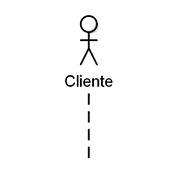
\includegraphics[width=0.45\columnwidth,height=0.35\textheight,keepaspectratio]{imagens/Fig7.1.png}
            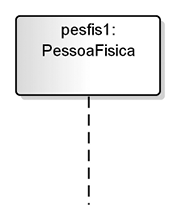
\includegraphics[width=0.45\columnwidth,height=0.35\textheight,keepaspectratio]{imagens/Fig7.2.png}
            \vspace{0.1cm}
            
            {\scriptsize \textbf{Lifeline de Ator (Fig. 7.1) e Objeto (Fig. 7.2 - Guedes)}}
        \end{column}
    \end{columns}
\end{frame}

% -----------------------------------------------------------------------------
% SLIDE 5: Tipos de Mensagens e Estímulos (Fig. 7.3 e 7.4)
% -----------------------------------------------------------------------------
\begin{frame}{Tipos de Mensagens e Estímulos na UML 2}
    \begin{columns}
        \begin{column}{0.52\textwidth}
            \textbf{Classificação Semântica das Mensagens:}
            \begin{itemize}\footnotesize
                \item \textbf{Síncrona ($\blacktriangleright$):} Seta preenchida. O remetente \textbf{bloqueia a execução} até a resposta.
                \item \textbf{Assíncrona ($\rightarrow$):} Seta aberta. O remetente despacha o sinal e prossegue imediatamente.
                \item \textbf{Resposta/Retorno ($\dashrightarrow$):} Linha tracejada com retorno do valor calculado.
                \item \textbf{Autochamada (\textit{Self-Call}):} Seta que retorna ao próprio objeto, gerando foco de controle empilhado.
            \end{itemize}
        \end{column}
        \begin{column}{0.48\textwidth}
            \centering
            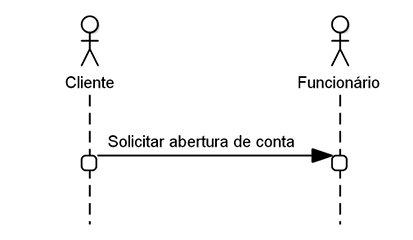
\includegraphics[width=\columnwidth,height=0.25\textheight,keepaspectratio]{imagens/Fig7.3.png}\\[0.05cm]
            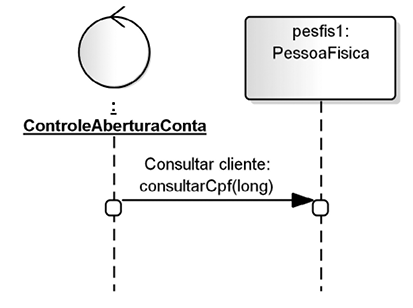
\includegraphics[width=\columnwidth,height=0.25\textheight,keepaspectratio]{imagens/Fig7.4.png}\\[0.05cm]
            {\tiny \textbf{Mensagens Síncronas (Fig. 7.3) e Autochamada (Fig. 7.4)}}
        \end{column}
    \end{columns}
\end{frame}

% -----------------------------------------------------------------------------
% SLIDE 6: Criação e Destruição de Instâncias (Fig. 7.5 e 7.7)
% -----------------------------------------------------------------------------
\begin{frame}{Criação e Destruição de Instâncias no Tempo}
    \begin{columns}
        \begin{column}{0.52\textwidth}
            \textbf{Mensagens Construtoras (\textit{Create}):}
            \begin{itemize}
                \item Mensagem com estereótipo \texttt{<<create>>} ou operação construtora (\texttt{new()});
                \item A seta aponta \textbf{diretamente para a caixa de cabeçalho} do novo objeto, indicando que ele não existia no início do cenário.
            \end{itemize}
            \vspace{0.2cm}
            \textbf{Mensagens Destrutoras (\textit{Destroy}):}
            \begin{itemize}
                \item Mensagem com estereótipo \texttt{<<destroy>>} ou invocação de destruição explícita;
                \item A linha de vida do objeto é encerrada com um grande \textbf{marcador em cruz ($\times$)}, indicando desalocação de memória.
            \end{itemize}
        \end{column}
        \begin{column}{0.48\textwidth}
            \centering
            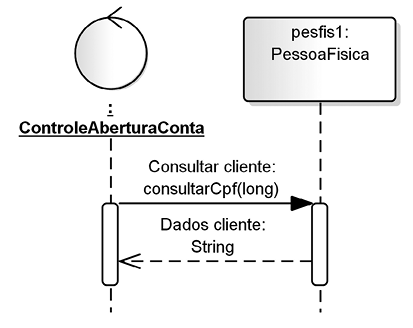
\includegraphics[width=\columnwidth,height=0.32\textheight,keepaspectratio]{imagens/Fig7.5.png}
            \vspace{0.1cm}
            
            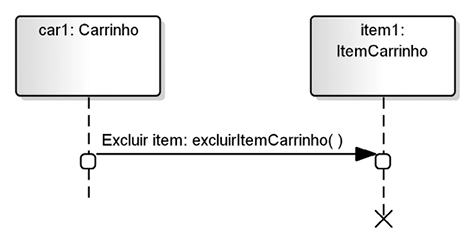
\includegraphics[width=\columnwidth,height=0.32\textheight,keepaspectratio]{imagens/Fig7.7.png}
            \vspace{0.1cm}
            
            {\scriptsize \textbf{Criação (Fig. 7.5) e Destruição com $\times$ (Fig. 7.7 - Guedes)}}
        \end{column}
    \end{columns}
\end{frame}

% -----------------------------------------------------------------------------
% SLIDE 7: Fragmentos Combinados: alt e opt (Fig. 7.8 e 7.9)
% -----------------------------------------------------------------------------
\begin{frame}{Fragmentos Combinados: Desvios Condicionais (\texttt{alt} e \texttt{opt})}
    \begin{columns}
        \begin{column}{0.52\textwidth}
            \textbf{Avanço da UML 2: Fragmentos Combinados}
            \begin{itemize}\footnotesize
                \item Caixas estruturadas com aba de operador no canto superior esquerdo e operandos delimitados.
            \end{itemize}
            \vspace{0.1cm}
            \textbf{Operadores de Desvio:}
            \begin{itemize}\footnotesize
                \item \textbf{Operador \texttt{alt} (\textit{Alternatives}):} Ramos mutuamente exclusivos (\texttt{if-else}) separados por linha tracejada com guardas \texttt{[condição]}.
                \item \textbf{Operador \texttt{opt} (\textit{Option}):} Bloco condicional simples (\texttt{if} sem \texttt{else}); dispara apenas se a guarda for verdadeira.
            \end{itemize}
        \end{column}
        \begin{column}{0.48\textwidth}
            \centering
            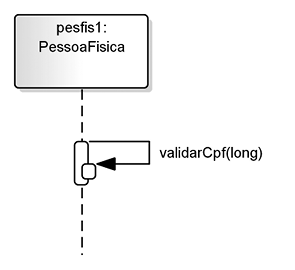
\includegraphics[width=\columnwidth,height=0.25\textheight,keepaspectratio]{imagens/Fig7.8.png}\\[0.05cm]
            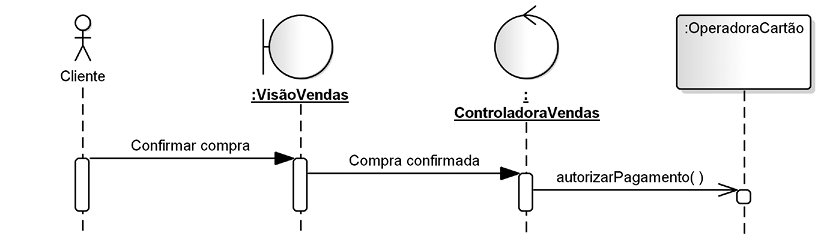
\includegraphics[width=\columnwidth,height=0.25\textheight,keepaspectratio]{imagens/Fig7.9.png}\\[0.05cm]
            {\tiny \textbf{Operador \texttt{alt} (Fig. 7.8) e Operador \texttt{opt} (Fig. 7.9)}}
        \end{column}
    \end{columns}
\end{frame}

% -----------------------------------------------------------------------------
% SLIDE 8: Fragmentos Combinados: loop, par e break (Fig. 7.10 e 7.11)
% -----------------------------------------------------------------------------
\begin{frame}{Fragmentos Combinados: Repetição, Paralelismo e Ruptura}
    \begin{columns}
        \begin{column}{0.52\textwidth}
            \textbf{Operador \texttt{loop} (Iteração):}
            \begin{itemize}
                \item Modela laços de repetição (\texttt{while}, \texttt{for});
                \item Notação com intervalo de contagem e guarda: \texttt{loop(min, max)[guarda]}, ex.: \texttt{loop(1, n)[temMaisItens]}.
            \end{itemize}
            \vspace{0.1cm}
            \textbf{Operador \texttt{par} (Paralelismo):}
            \begin{itemize}
                \item Define subcenários concorrentes executados em paralelo por diferentes threads.
            \end{itemize}
            \vspace{0.1cm}
            \textbf{Operador \texttt{break} (Ruptura / Exceção):}
            \begin{itemize}
                \item Executado em situações anormais (exceções), abandonando o fluxo restante do fragmento pai.
            \end{itemize}
        \end{column}
        \begin{column}{0.48\textwidth}
            \centering
            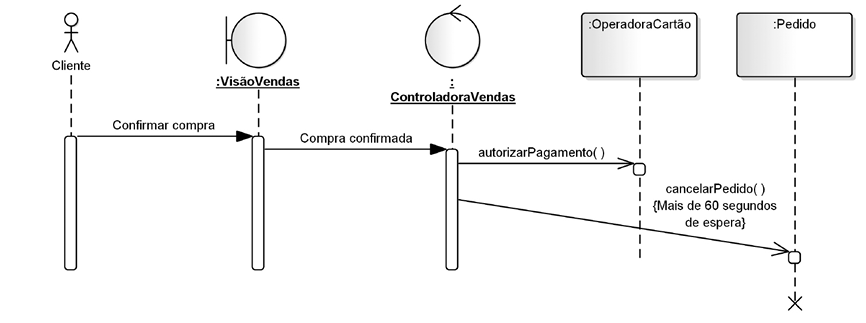
\includegraphics[width=\columnwidth,height=0.32\textheight,keepaspectratio]{imagens/Fig7.10.png}
            \vspace{0.1cm}
            
            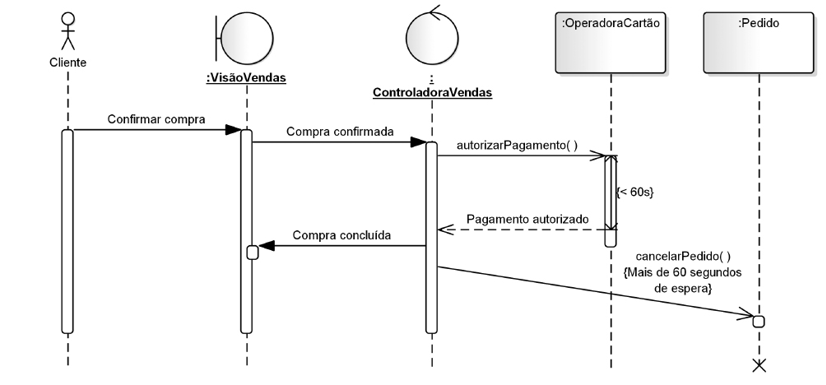
\includegraphics[width=\columnwidth,height=0.32\textheight,keepaspectratio]{imagens/Fig7.11.png}
            \vspace{0.1cm}
            
            {\scriptsize \textbf{Operador \texttt{loop} (Fig. 7.10) e Operador \texttt{par} (Fig. 7.11)}}
        \end{column}
    \end{columns}
\end{frame}

% -----------------------------------------------------------------------------
% SLIDE 9: Recursos Avançados: Invariantes, ref e Portões (Fig. 7.13 e 7.15)
% -----------------------------------------------------------------------------
\begin{frame}{Recursos Avançados de Sequência (Fig. 7.13 e 7.15)}
    \begin{columns}
        \begin{column}{0.52\textwidth}
            \textbf{Invariante de Estado (\textit{StateInvariant}):}
            \begin{itemize}
                \item Símbolo de retângulo arredondado sobreposto à linha de vida contendo uma restrição ou estado formal (ex.: \texttt{\{saldo >= 0\}});
                \item Deve ser obrigatoriamente verdadeiro para que o objeto possa receber mensagens naquele instante.
            \end{itemize}
            \vspace{0.2cm}
            \textbf{Uso de Interação (\texttt{ref}):}
            \begin{itemize}
                \item Permite modularizar o diagrama, inserindo uma referência a outro Diagrama de Sequência já especificado (evita duplicação de diagramas longos).
            \end{itemize}
        \end{column}
        \begin{column}{0.48\textwidth}
            \centering
            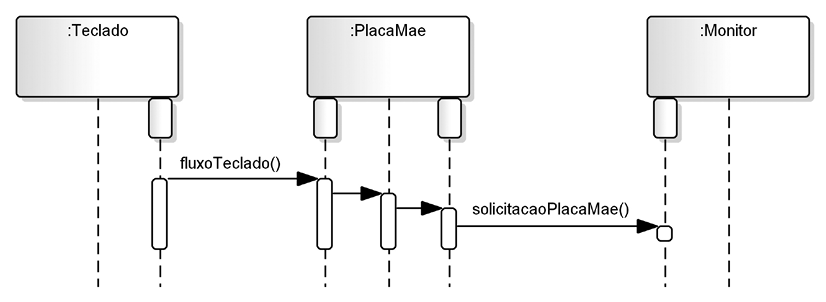
\includegraphics[width=\columnwidth,height=0.32\textheight,keepaspectratio]{imagens/Fig7.13.png}
            \vspace{0.1cm}
            
            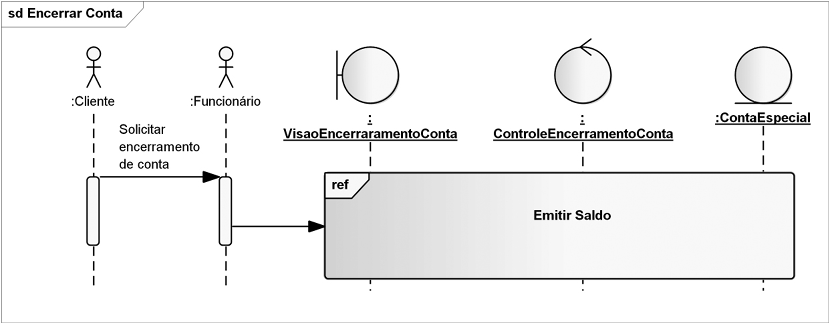
\includegraphics[width=\columnwidth,height=0.32\textheight,keepaspectratio]{imagens/Fig7.15.png}
            \vspace{0.1cm}
            
            {\scriptsize \textbf{Invariante de Estado (Fig. 7.13) e Operador \texttt{ref} (Fig. 7.15)}}
        \end{column}
    \end{columns}
\end{frame}

% -----------------------------------------------------------------------------
% SLIDE 10: Persistência e Padrões Repository / DAO (Fig. 7.22 e 7.23)
% -----------------------------------------------------------------------------
\begin{frame}{Integração com Persistência: Padrões Repository e DAO}
    \begin{columns}
        \begin{column}{0.52\textwidth}
            \textbf{O Papel da Camada de Dados na Sequência:}
            \begin{itemize}
                \item Na arquitetura em camadas (MVC/ECB), os objetos da camada de controle não executam SQL diretamente.
                \item O controller delega a persistência para uma instância \textbf{Repository} ou \textbf{DAO} (\textit{Data Access Object}).
                \item A classe Repository monta a entidade a partir do banco e retorna instâncias prontas para as camadas superiores.
                \item O Diagrama de Sequência documenta com clareza o ciclo de leitura, validação e gravação no banco de dados.
            \end{itemize}
        \end{column}
        \begin{column}{0.48\textwidth}
            \centering
            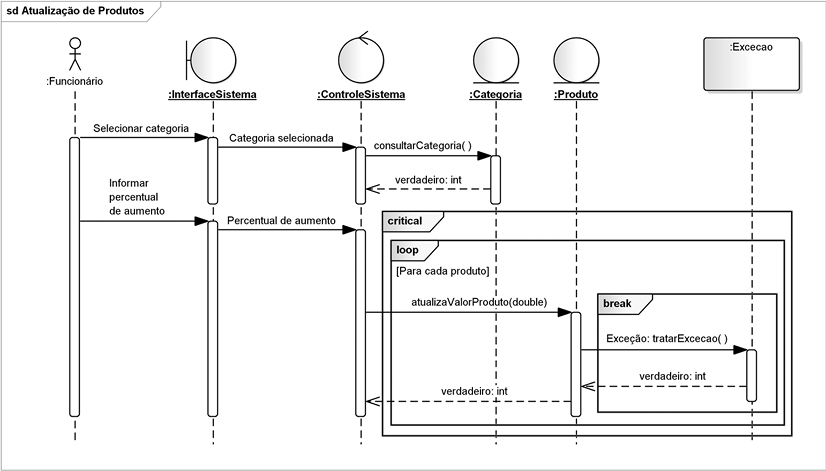
\includegraphics[width=\columnwidth,height=0.32\textheight,keepaspectratio]{imagens/Fig7.22.png}
            \vspace{0.1cm}
            
            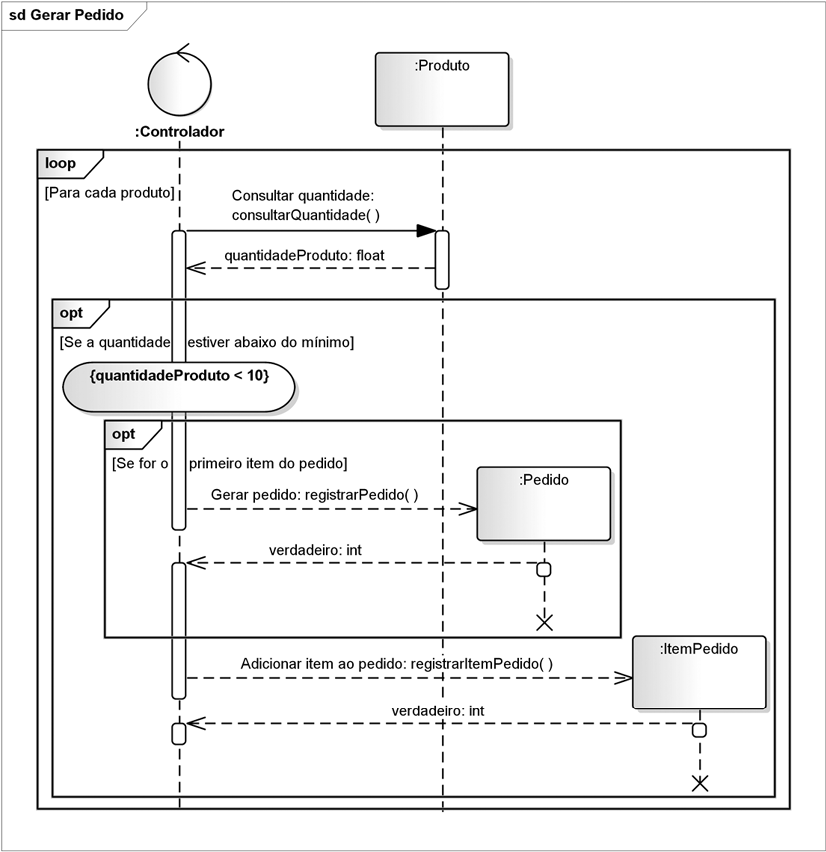
\includegraphics[width=\columnwidth,height=0.32\textheight,keepaspectratio]{imagens/Fig7.23.png}
            \vspace{0.1cm}
            
            {\scriptsize \textbf{Chamadas a DAO e Repository no Diagrama de Sequência (Guedes)}}
        \end{column}
    \end{columns}
\end{frame}

% -----------------------------------------------------------------------------
% SLIDE 11: Estudo de Caso Bancário: Sequência de Saque (Fig. 7.18)
% -----------------------------------------------------------------------------
\begin{frame}{Estudo de Caso Bancário: Realizar Saque na Sequência}
    \begin{columns}
        \begin{column}{0.45\textwidth}
            \textbf{Rastreamento do Fluxo:}
            \begin{enumerate}
                \item O cliente aciona \texttt{efetuarSaque(num, senha, valor)} na tela (\texttt{<<boundary>>});
                \item O controle valida a senha da conta;
                \item O fragmento \texttt{alt} avalia o saldo:
                \begin{itemize}
                    \item Se \texttt{saldo >= valor}: debita na conta, emite cédulas e grava log de movimento;
                    \item Senão (\texttt{else}): informa mensagem de saldo insuficiente ao cliente.
                \end{itemize}
            \end{enumerate}
        \end{column}
        \begin{column}{0.55\textwidth}
            \centering
            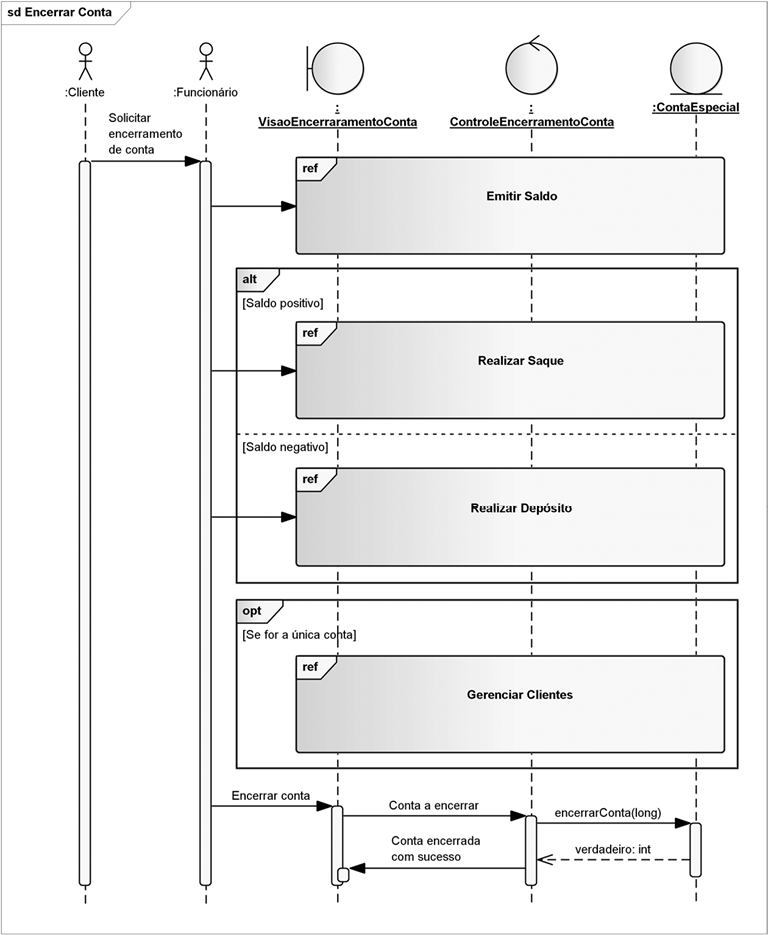
\includegraphics[width=\columnwidth,height=0.55\textheight,keepaspectratio]{imagens/Fig7.18.png}
            \vspace{0.1cm}
            
            {\scriptsize \textbf{Processo de Saque Bancário no Diagrama de Sequência (Fig. 7.18 - Guedes)}}
        \end{column}
    \end{columns}
\end{frame}

% =============================================================================
\section{Diagrama de Comunicação (Capítulo 8)}
% =============================================================================

% -----------------------------------------------------------------------------
% SLIDE 12: Introdução ao Diagrama de Comunicação (Fig. 8.1 e 8.2)
% -----------------------------------------------------------------------------
\begin{frame}{Introdução ao Diagrama de Comunicação (Cap. 8)}
    \begin{columns}
        \begin{column}{0.52\textwidth}
            \textbf{Origem e Propósito:}
            \begin{itemize}
                \item Chamado de \textit{Diagrama de Colaboração} na UML 1.x;
                \item É o segundo diagrama de interação da UML 2.
                \item Possui \textbf{equivalência semântica} com o Diagrama de Sequência, expressando as mesmas mensagens.
            \end{itemize}
            \vspace{0.2cm}
            \textbf{Mudança Fundamental de Perspectiva:}
            \begin{itemize}
                \item Em vez de uma linha do tempo vertical, os objetos são dispostos como nós em uma \textbf{rede de conexões};
                \item Enfatiza os \textbf{vínculos estruturais (\textit{links})} que possibilitam a comunicação entre as partes.
            \end{itemize}
        \end{column}
        \begin{column}{0.48\textwidth}
            \centering
            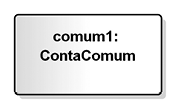
\includegraphics[width=0.45\columnwidth,height=0.35\textheight,keepaspectratio]{imagens/Fig8.1.png}
            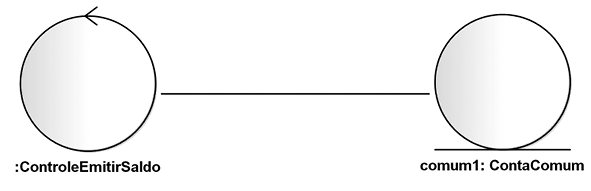
\includegraphics[width=0.45\columnwidth,height=0.35\textheight,keepaspectratio]{imagens/Fig8.2.png}
            \vspace{0.1cm}
            
            {\scriptsize \textbf{Lifeline (Fig. 8.1) e Vínculo com Mensagem (Fig. 8.2 - Guedes)}}
        \end{column}
    \end{columns}
\end{frame}

% -----------------------------------------------------------------------------
% SLIDE 13: Mensagens e Numeração Sequencial Hierárquica (Fig. 8.3 e 8.4)
% -----------------------------------------------------------------------------
\begin{frame}{Numeração Hierárquica e Aninhamento de Mensagens}
    \begin{columns}
        \begin{column}{0.52\textwidth}
            \textbf{Ordenação Temporal via Numeração:}
            \begin{itemize}\footnotesize
                \item A sequência temporal é governada por \textbf{numeração decimal aninhada};
                \item Pequenas setas ao lado do vínculo indicam a direção.
            \end{itemize}
            \vspace{0.1cm}
            \textbf{Hierarquia de Aninhamento:}
            \begin{itemize}\footnotesize
                \item \texttt{1: operacao()}: Mensagem inicial disparada;
                \item \texttt{1.1: subOpA()}: Chamada decorrente de \texttt{1};
                \item \texttt{1.2: subOpB()}: Segunda suboperação no escopo;
                \item \texttt{1.2.1: detalhe()}: Chamada aninhada de \texttt{1.2}.
            \end{itemize}
        \end{column}
        \begin{column}{0.48\textwidth}
            \centering
            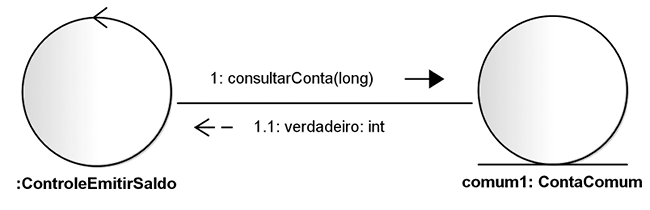
\includegraphics[width=\columnwidth,height=0.24\textheight,keepaspectratio]{imagens/Fig8.3.png}\\[0.05cm]
            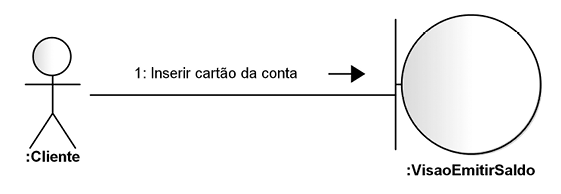
\includegraphics[width=\columnwidth,height=0.24\textheight,keepaspectratio]{imagens/Fig8.4.png}\\[0.05cm]
            {\tiny \textbf{Mensagens Aninhadas (Fig. 8.3 e 8.4 - Guedes)}}
        \end{column}
    \end{columns}
\end{frame}

% -----------------------------------------------------------------------------
% SLIDE 14: Autochamada, Guardas e Iterações (Fig. 8.5 e 8.8)
% -----------------------------------------------------------------------------
\begin{frame}{Autochamada, Condições de Guarda e Iterações}
    \begin{columns}
        \begin{column}{0.52\textwidth}
            \textbf{Autochamada (\textit{Self-Call}):}
            \begin{itemize}
                \item Representada por um vínculo em arco ou laço que sai e retorna para o próprio objeto (Fig. 8.5).
            \end{itemize}
            \vspace{0.1cm}
            \textbf{Condições de Guarda:}
            \begin{itemize}
                \item Expressas entre colchetes antes do nome da operação, ex.: \texttt{1.1: [saldo >= valor] debitar()}.
            \end{itemize}
            \vspace{0.1cm}
            \textbf{Expressão de Iteração (Laços):}
            \begin{itemize}
                \item Um asterisco (\texttt{*}) denota repetição sobre múltiplos elementos;
                \item Sintaxe completa: \texttt{* [i := 1..n]: calcularSubtotal()}.
            \end{itemize}
        \end{column}
        \begin{column}{0.48\textwidth}
            \centering
            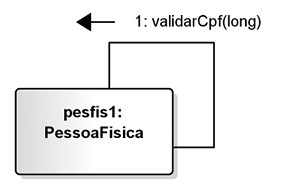
\includegraphics[width=\columnwidth,height=0.32\textheight,keepaspectratio]{imagens/Fig8.5.png}
            \vspace{0.1cm}
            
            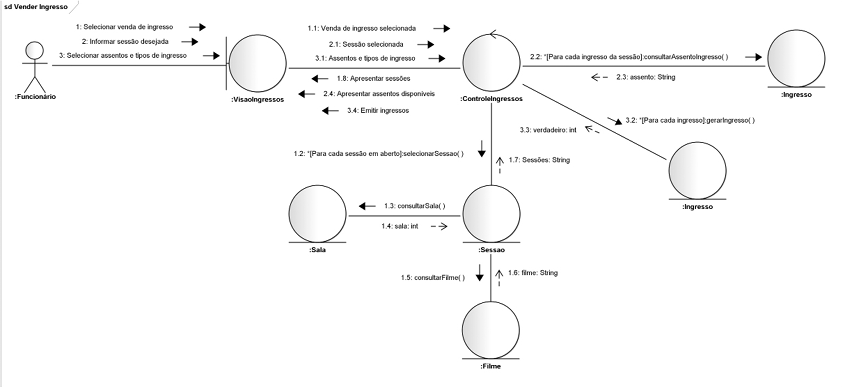
\includegraphics[width=\columnwidth,height=0.32\textheight,keepaspectratio]{imagens/Fig8.8.png}
            \vspace{0.1cm}
            
            {\scriptsize \textbf{Autochamada (Fig. 8.5) e Laço de Iteração (Fig. 8.8 - Guedes)}}
        \end{column}
    \end{columns}
\end{frame}

% -----------------------------------------------------------------------------
% SLIDE 15: Estudo de Caso Bancário: Comunicação no Emitir Saldo (Fig. 8.7)
% -----------------------------------------------------------------------------
\begin{frame}{Estudo de Caso: Comunicação no Processo Emitir Saldo}
    \begin{columns}
        \begin{column}{0.5\textwidth}
            \textbf{Análise do Fluxo na Rede de Objetos:}
            \begin{itemize}
                \item \texttt{1: emitirSaldo()}: Cliente solicita na interface \texttt{TelaEmitirSaldo};
                \item \texttt{1.1: validaSenha()}: O controle aciona a conta bancária;
                \item \texttt{1.2: [senhaCorreta] obterSaldo()}: A conta calcula e retorna o saldo derivado;
                \item \texttt{1.3: exibirSaldo()}: A tela apresenta os dados ao cliente.
            \end{itemize}
            \vspace{0.2cm}
            \textbf{Vantagem Visual:}
            Fica imediatamente claro quais instâncias dependem diretamente de quem para trocar dados.
        \end{column}
        \begin{column}{0.5\textwidth}
            \centering
            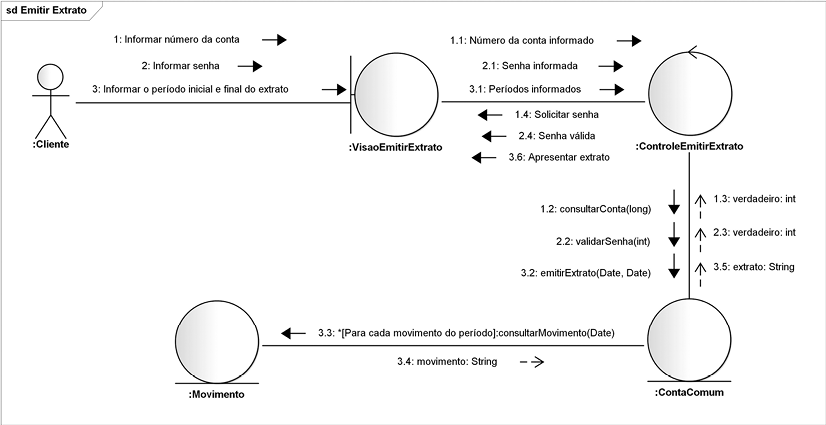
\includegraphics[width=\columnwidth,height=0.55\textheight,keepaspectratio]{imagens/Fig8.7.png}
            \vspace{0.1cm}
            
            {\scriptsize \textbf{Diagrama de Comunicação do Processo Emitir Saldo (Fig. 8.7 - Guedes)}}
        \end{column}
    \end{columns}
\end{frame}

% -----------------------------------------------------------------------------
% SLIDE 16: Análise Comparativa: Sequência vs. Comunicação
% -----------------------------------------------------------------------------
\begin{frame}{Análise Comparativa: Sequência vs. Comunicação}
    \begin{table}
        \centering
        \scriptsize
        \begin{tabular}{p{3.2cm} p{3.8cm} p{3.8cm}}
            \toprule
            \textbf{Característica} & \textbf{Diagrama de Sequência} & \textbf{Diagrama de Comunicação} \\
            \midrule
            \textbf{Foco Principal} & Ordenação temporal e cronologia de execução. & Topologia de rede e vínculos estruturais. \\
            \addlinespace
            \textbf{Representação do Tempo} & Eixo vertical contínuo (de cima para baixo). & Numeração sequencial aninhada (\texttt{1.1}, \texttt{1.2}). \\
            \addlinespace
            \textbf{Foco de Controle / Ativação} & Barras verticais detalhadas e explícitas. & Não representa visualmente o tempo de bloqueio. \\
            \addlinespace
            \textbf{Complexidade de Desvios} & Fragmentos elegantes (\texttt{alt}, \texttt{loop}, \texttt{par}). & Guardas em linha e laços com \texttt{*}. \\
            \addlinespace
            \textbf{Melhor Cenário de Uso} & Documentar cenários complexos de Casos de Uso. & Validar coesão e acoplamento entre classes. \\
            \bottomrule
        \end{tabular}
        \caption{Quadro comparativo dos Diagramas de Interação (Capítulos 7 e 8 - Guedes).}
    \end{table}
\end{frame}

% -----------------------------------------------------------------------------
% SLIDE 17: Equivalência Semântica e Regras de Conversão
% -----------------------------------------------------------------------------
\begin{frame}{Equivalência Semântica e Regras de Conversão}
    \begin{columns}
        \begin{column}{0.55\textwidth}
            \textbf{Como Converter Sequência em Comunicação:}
            \begin{enumerate}
                \item Converta cada linha de vida em um objeto nó no diagrama de comunicação;
                \item Crie um vínculo sólido entre pares de nós para cada mensagem trocada;
                \item Atribua numeração decimal correspondente ao nível de aninhamento dos focos de controle da sequência;
                \item Adicione a seta direcional indicando remetente $\rightarrow$ destinatário.
            \end{enumerate}
        \end{column}
        \begin{column}{0.45\textwidth}
            \begin{block}{Regra de Ouro da UML 2}
                Ambos os diagramas expressam \textbf{exatamente o mesmo comportamento}. A escolha depende exclusivamente do aspecto que o engenheiro deseja destacar para a equipe de desenvolvimento.
            \end{block}
        \end{column}
    \end{columns}
\end{frame}

% =============================================================================
\section{Diagrama de Máquina de Estados (Capítulo 9)}
% =============================================================================

% -----------------------------------------------------------------------------
% SLIDE 18: Introdução ao Diagrama de Máquina de Estados (Fig. 9.1, 9.2, 9.3)
% -----------------------------------------------------------------------------
\begin{frame}{Introdução ao Diagrama de Máquina de Estados (Cap. 9)}
    \begin{columns}
        \begin{column}{0.52\textwidth}
            \textbf{Conceito de Estado e Ciclo de Vida:}
            \begin{itemize}\footnotesize
                \item Condição na qual uma entidade \textbf{satisfaz determinada restrição}, executa ações ou aguarda eventos.
                \item Foca no \textbf{ciclo de vida de uma única classe reativa} (ex.: \texttt{Pedido}, \texttt{ContaComum}).
            \end{itemize}
            \vspace{0.1cm}
            \textbf{Elementos Fundamentais:}
            \begin{itemize}\footnotesize
                \item \textbf{Estado Inicial ($\bullet$):} Ponto de partida do ciclo;
                \item \textbf{Estado Simples:} Retângulo de cantos arredondados;
                \item \textbf{Estado Final ($\odot$):} Encerramento da vida da instância.
            \end{itemize}
        \end{column}
        \begin{column}{0.48\textwidth}
            \centering
            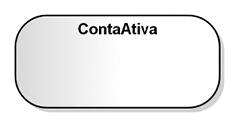
\includegraphics[width=0.85\columnwidth,height=0.20\textheight,keepaspectratio]{imagens/Fig9.1.png}\\[0.05cm]
            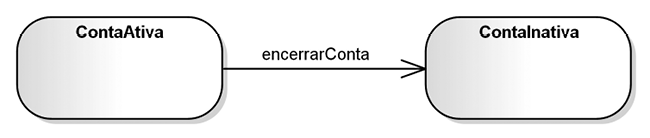
\includegraphics[width=0.38\columnwidth,height=0.15\textheight,keepaspectratio]{imagens/Fig9.2.png}
            \hspace{0.2cm}
            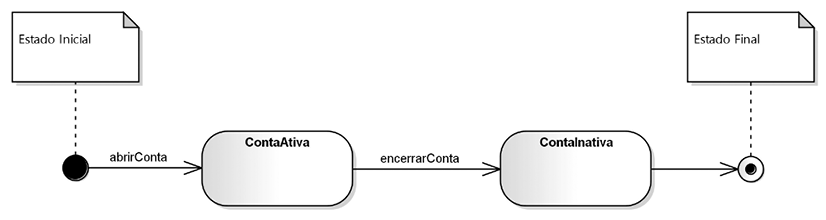
\includegraphics[width=0.38\columnwidth,height=0.15\textheight,keepaspectratio]{imagens/Fig9.3.png}\\[0.05cm]
            {\tiny \textbf{Estado Simples (Fig. 9.1), Inicial (9.2) e Final (9.3)}}
        \end{column}
    \end{columns}
\end{frame}

% -----------------------------------------------------------------------------
% SLIDE 19: Transições Dirigidas por Eventos e Guardas (Fig. 9.4 e 9.5)
% -----------------------------------------------------------------------------
\begin{frame}{Transições Dirigidas por Eventos e Sintaxe Canônica}
    \begin{columns}
        \begin{column}{0.52\textwidth}
            \textbf{A Fórmula Canônica da Transição UML 2:}
            \begin{center}
                \large\texttt{\textbf{gatilho [guarda] / acao}}
            \end{center}
            \vspace{0.05cm}
            \textbf{Partes Constituintes:}
            \begin{itemize}\footnotesize
                \item \textbf{Gatilho / Evento (\textit{Trigger}):} Estímulo que dispara a transição (ex.: \texttt{pagtoAprovado}).
                \item \textbf{Condição de Guarda (\textit{Guard}):} Expressão lógica entre colchetes. Se falsa, bloqueia o disparo (ex.: \texttt{[valor > 0]}).
                \item \textbf{Ação de Efeito (\textit{Effect}):} Comportamento atômico instantâneo executado na transição (ex.: \texttt{/ emitirRecibo()}).
            \end{itemize}
        \end{column}
        \begin{column}{0.48\textwidth}
            \centering
            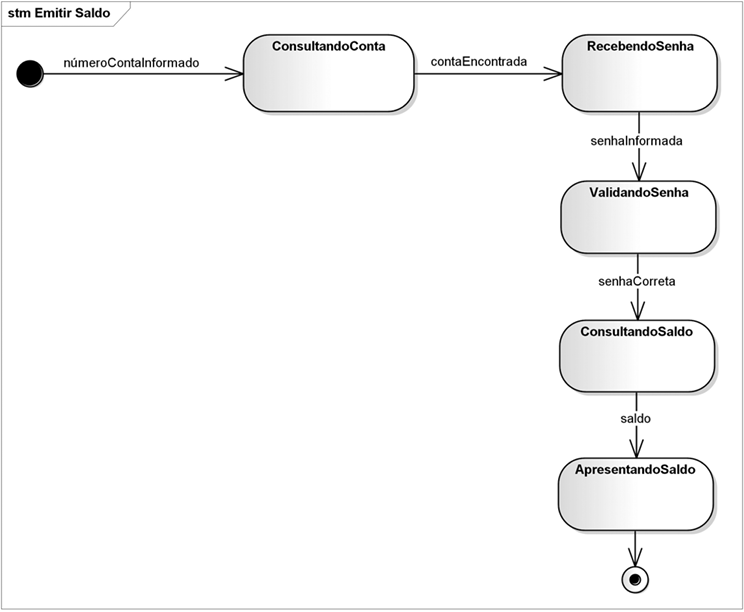
\includegraphics[width=\columnwidth,height=0.25\textheight,keepaspectratio]{imagens/Fig9.4.png}\\[0.05cm]
            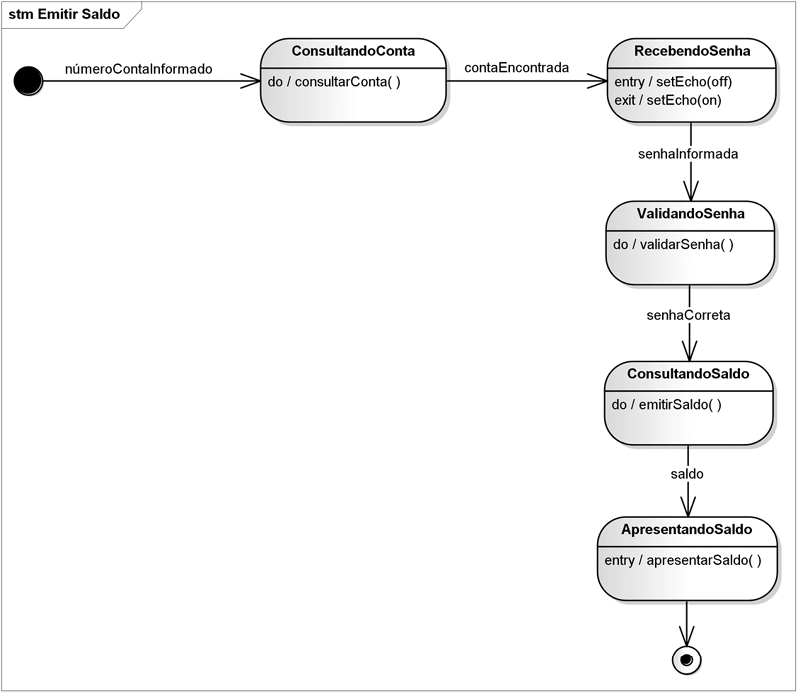
\includegraphics[width=\columnwidth,height=0.25\textheight,keepaspectratio]{imagens/Fig9.5.png}\\[0.05cm]
            {\tiny \textbf{Sintaxe de Transição e Guardas (Fig. 9.4 e 9.5 - Guedes)}}
        \end{column}
    \end{columns}
\end{frame}

% -----------------------------------------------------------------------------
% SLIDE 20: Atividades Internas do Estado: entry, do, exit (Fig. 9.6)
% -----------------------------------------------------------------------------
\begin{frame}{Atividades Internas do Estado (\texttt{entry}, \texttt{do}, \texttt{exit})}
    \begin{columns}
        \begin{column}{0.55\textwidth}
            \textbf{Comportamentos Internos do Estado:}
            \begin{itemize}\footnotesize
                \item \textbf{\texttt{entry / acao}:} Execução atômica instantânea \textbf{ao entrar} no estado.
                \item \textbf{\texttt{do / atividade}:} Execução contínua \textbf{enquanto permanece} no estado (interrompível por eventos).
                \item \textbf{\texttt{exit / acao}:} Execução atômica \textbf{ao deixar} o estado.
            \end{itemize}
            \vspace{0.1cm}
            \textbf{Exemplo Prático (\texttt{EM\_ROTA}):}
            \begin{itemize}\scriptsize
                \item \texttt{entry / iniciarTelemetriaGps()}
                \item \texttt{do / transmitirCoordenadas()}
                \item \texttt{exit / finalizarRastreamento()}
            \end{itemize}
        \end{column}
        \begin{column}{0.45\textwidth}
            \centering
            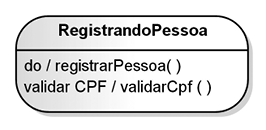
\includegraphics[width=0.9\columnwidth,height=0.40\textheight,keepaspectratio]{imagens/Fig9.6.png}\\[0.05cm]
            {\tiny \textbf{Atividades Internas (Fig. 9.6 - Guedes)}}
        \end{column}
    \end{columns}
\end{frame}

% -----------------------------------------------------------------------------
% SLIDE 21: Transições Internas vs. Autotransições (Fig. 9.7 e 9.8)
% -----------------------------------------------------------------------------
\begin{frame}{Transições Internas vs. Autotransições}
    \begin{columns}
        \begin{column}{0.52\textwidth}
            \textbf{Transição Interna (Fig. 9.7):}
            \begin{itemize}
                \item Responde a um evento alterando variáveis internas, mas \textbf{não provoca saída nem reentrada no estado}.
                \item \textbf{Ações \texttt{entry} e \texttt{exit} NÃO são disparadas}.
            \end{itemize}
            \vspace{0.2cm}
            \textbf{Autotransição (Fig. 9.8):}
            \begin{itemize}
                \item Seta sai do contorno do estado e aponta de volta para o próprio estado.
                \item Provoca a saída formal e reentrada imediata.
                \item \textbf{Dispara \texttt{exit} e depois executa \texttt{entry} novamente}.
            \end{itemize}
        \end{column}
        \begin{column}{0.48\textwidth}
            \centering
            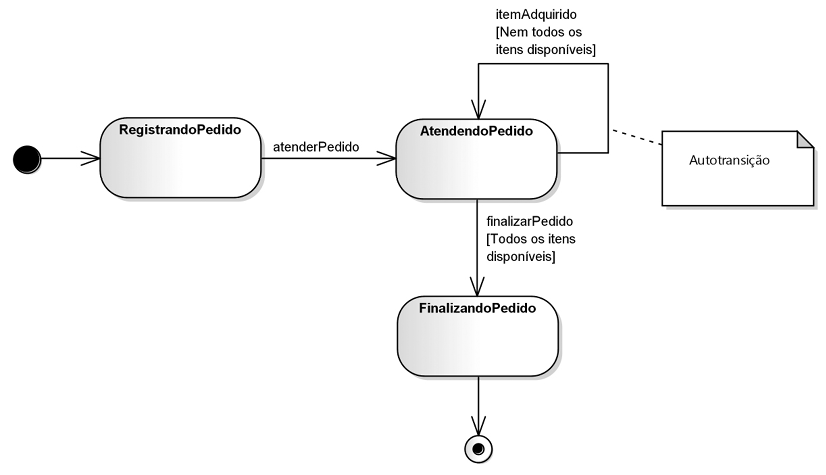
\includegraphics[width=\columnwidth,height=0.32\textheight,keepaspectratio]{imagens/Fig9.7.png}
            \vspace{0.1cm}
            
            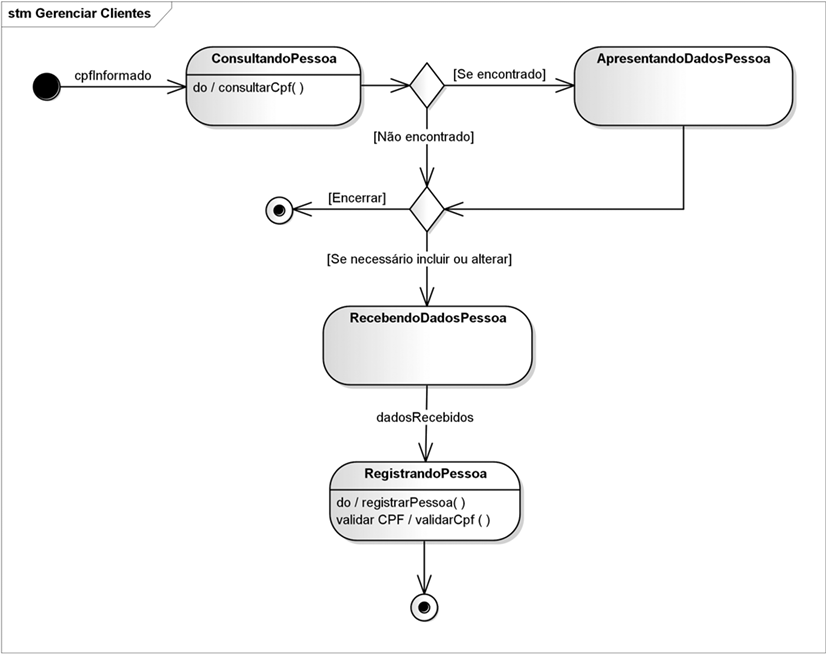
\includegraphics[width=\columnwidth,height=0.32\textheight,keepaspectratio]{imagens/Fig9.8.png}
            \vspace{0.1cm}
            
            {\scriptsize \textbf{Transição Interna (Fig. 9.7) vs. Autotransição (Fig. 9.8 - Guedes)}}
        \end{column}
    \end{columns}
\end{frame}

% -----------------------------------------------------------------------------
% SLIDE 22: Pseudoestados de Decisão: Escolha vs. Junção (Fig. 9.9 e 9.16)
% -----------------------------------------------------------------------------
\begin{frame}{Pseudoestados de Decisão: Escolha (\textit{Choice}) vs. Junção (\textit{Junction})}
    \begin{columns}
        \begin{column}{0.52\textwidth}
            \textbf{Escolha (\textit{Choice} - $\lozenge$):}
            \begin{itemize}\footnotesize
                \item Representado por um losango (Fig. 9.9);
                \item \textbf{Avaliação dinâmica em runtime}: as guardas são avaliadas quando o fluxo alcança o vértice;
                \item Suporta ramo padrão \texttt{[else]}.
            \end{itemize}
            \vspace{0.1cm}
            \textbf{Junção (\textit{Junction} - $\bullet$):}
            \begin{itemize}\footnotesize
                \item Círculo sólido menor que o estado inicial (Fig. 9.16);
                \item \textbf{Avaliação estática preliminar}: todas as guardas são avaliadas antes do disparo da transição.
            \end{itemize}
        \end{column}
        \begin{column}{0.48\textwidth}
            \centering
            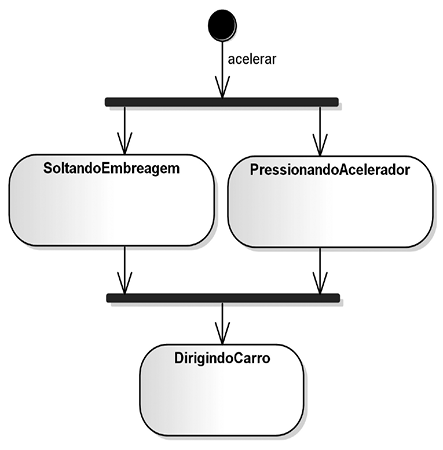
\includegraphics[width=\columnwidth,height=0.23\textheight,keepaspectratio]{imagens/Fig9.9.png}\\[0.05cm]
            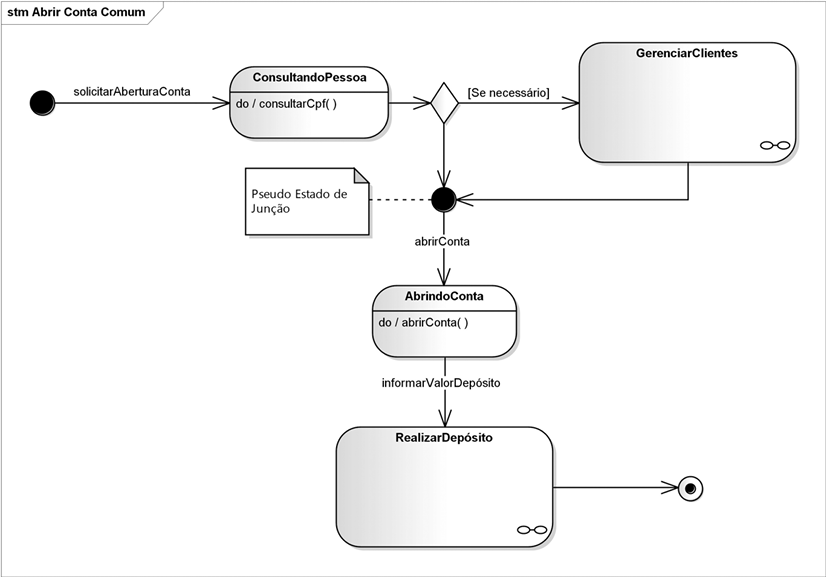
\includegraphics[width=\columnwidth,height=0.23\textheight,keepaspectratio]{imagens/Fig9.16.png}\\[0.05cm]
            {\tiny \textbf{Escolha (Fig. 9.9) e Junção (Fig. 9.16 - Guedes)}}
        \end{column}
    \end{columns}
\end{frame}

% -----------------------------------------------------------------------------
% SLIDE 23: Pseudoestados de Concorrência e Histórico (Fig. 9.10 e 9.12)
% -----------------------------------------------------------------------------
\begin{frame}{Bifurcação/União (\textit{Fork/Join}) e Pseudoestado Histórico}
    \begin{columns}
        \begin{column}{0.52\textwidth}
            \textbf{Bifurcação / União (\textit{Fork/Join}):}
            \begin{itemize}
                \item Barra espessa horizontal ou vertical dividindo uma transição em duas ou sincronizando ramos paralelos.
            \end{itemize}
            \vspace{0.1cm}
            \textbf{Pseudoestado de Histórico ($H$ e $H^*$):}
            \begin{itemize}
                \item Permite a um estado composto \textbf{lembrar o último subestado ativo} antes de ter sido interrompido por uma transição externa.
                \item \textbf{Histórico Raso ($H$):} Restaura apenas o subestado do primeiro nível hierárquico.
                \item \textbf{Histórico Profundo ($H^*$):} Restaura o subestado em qualquer nível de profundidade recursiva.
            \end{itemize}
        \end{column}
        \begin{column}{0.48\textwidth}
            \centering
            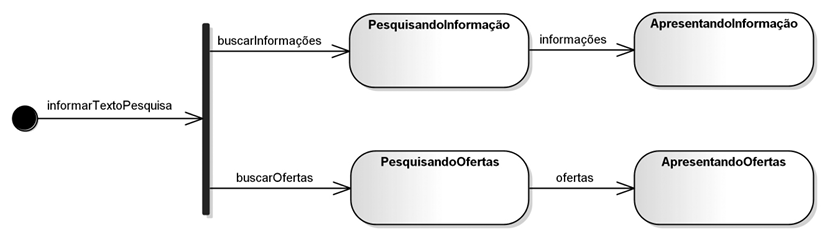
\includegraphics[width=\columnwidth,height=0.32\textheight,keepaspectratio]{imagens/Fig9.10.png}
            \vspace{0.1cm}
            
            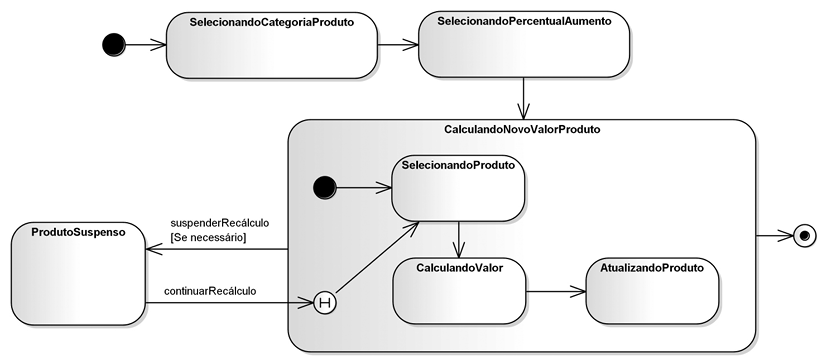
\includegraphics[width=\columnwidth,height=0.32\textheight,keepaspectratio]{imagens/Fig9.12.png}
            \vspace{0.1cm}
            
            {\scriptsize \textbf{Fork/Join (Fig. 9.10) e Pseudoestado de Histórico (Fig. 9.12)}}
        \end{column}
    \end{columns}
\end{frame}

% -----------------------------------------------------------------------------
% SLIDE 24: Estados Compostos e Estados Compostos Ortogonais (Fig. 9.11 e 9.14)
% -----------------------------------------------------------------------------
\begin{frame}{Estados Compostos e Regiões Ortogonais}
    \begin{columns}
        \begin{column}{0.52\textwidth}
            \textbf{Estados Compostos (Subestados):}
            \begin{itemize}
                \item Um estado simples pode conter uma máquina de estados inteira aninhada dentro de si (Fig. 9.11).
                \item Facilita a abstração de sistemas complexos.
            \end{itemize}
            \vspace{0.1cm}
            \textbf{Estados Ortogonais (Concorrência):}
            \begin{itemize}
                \item O estado composto é dividido em duas ou mais regiões separadas por uma \textbf{linha pontilhada} (Fig. 9.14);
                \item O objeto está simultaneamente em um subestado de cada região ao mesmo tempo.
            \end{itemize}
        \end{column}
        \begin{column}{0.48\textwidth}
            \centering
            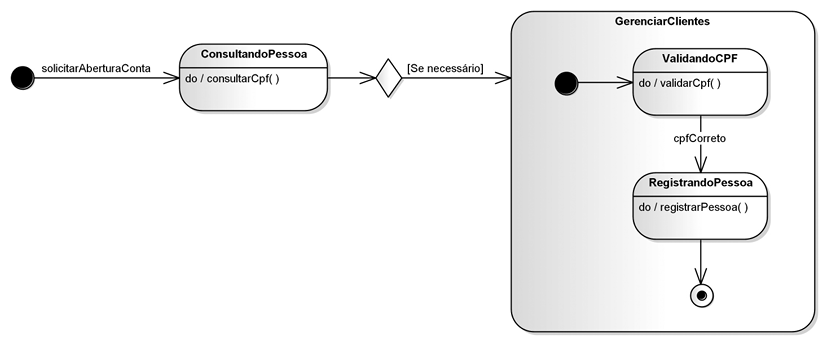
\includegraphics[width=\columnwidth,height=0.32\textheight,keepaspectratio]{imagens/Fig9.11.png}
            \vspace{0.1cm}
            
            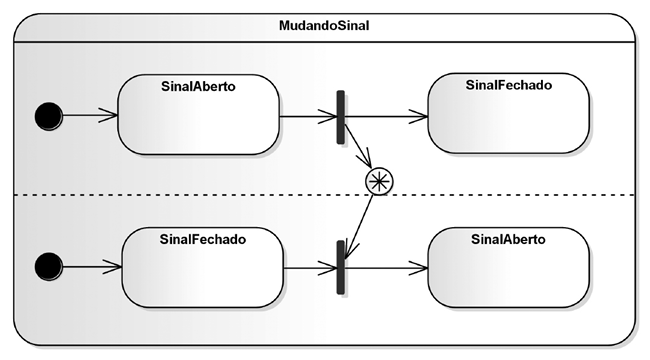
\includegraphics[width=\columnwidth,height=0.32\textheight,keepaspectratio]{imagens/Fig9.14.png}
            \vspace{0.1cm}
            
            {\scriptsize \textbf{Estados Compostos (Fig. 9.11) e Ortogonais (Fig. 9.14)}}
        \end{column}
    \end{columns}
\end{frame}

% -----------------------------------------------------------------------------
% SLIDE 25: Pseudoestados Especiais e Pontos de Conexão (Fig. 9.17 e 9.18)
% -----------------------------------------------------------------------------
\begin{frame}{Pseudoestados Especiais e Término}
    \begin{columns}
        \begin{column}{0.52\textwidth}
            \textbf{Estado de Submáquina:}
            \begin{itemize}
                \item Referencia uma máquina de estados externa reutilizável, indicada pelo símbolo de dois retângulos conectados no canto.
            \end{itemize}
            \vspace{0.1cm}
            \textbf{Ponto de Entrada e Ponto de Saída:}
            \begin{itemize}
                \item Círculos na borda do estado composto permitindo saltar diretamente para subestados específicos.
            \end{itemize}
            \vspace{0.1cm}
            \textbf{Pseudoestado de Término ($\bigotimes$):}
            \begin{itemize}
                \item Círculo com um \textbf{X} interno. Destrói o objeto imediatamente, sem disparar ações \texttt{exit}.
            \end{itemize}
        \end{column}
        \begin{column}{0.48\textwidth}
            \centering
            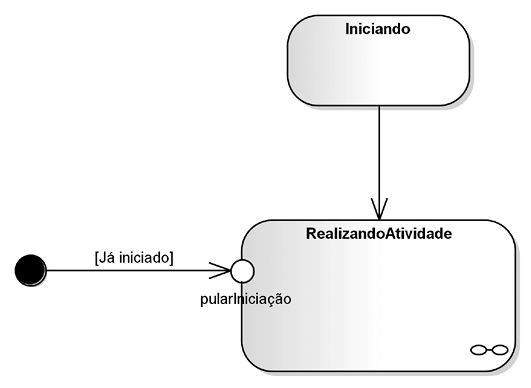
\includegraphics[width=0.45\columnwidth,height=0.35\textheight,keepaspectratio]{imagens/Fig9.17.png}
            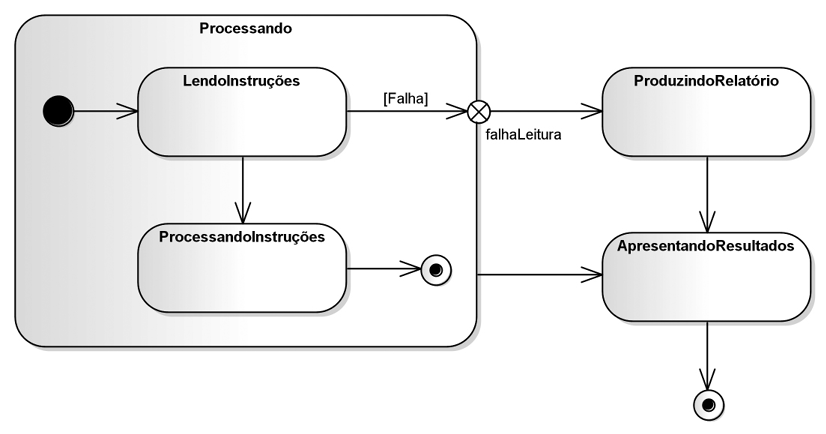
\includegraphics[width=0.45\columnwidth,height=0.35\textheight,keepaspectratio]{imagens/Fig9.18.png}
            \vspace{0.1cm}
            
            {\scriptsize \textbf{Pontos de Entrada/Saída (Fig. 9.17) e Término (Fig. 9.18)}}
        \end{column}
    \end{columns}
\end{frame}

% -----------------------------------------------------------------------------
% SLIDE 26: Estudo de Caso Bancário: Máquina de Estados da ContaComum (Fig. 9.28)
% -----------------------------------------------------------------------------
\begin{frame}{Estudo de Caso: Ciclo de Vida da Conta Bancária}
    \begin{columns}
        \begin{column}{0.48\textwidth}
            \textbf{Ciclo de Vida de uma Conta Bancária:}
            \begin{itemize}
                \item \textbf{Cadastrada:} Aguardando primeiro depósito;
                \item \textbf{Ativa:} Operando normalmente com saques e depósitos;
                \item \textbf{Bloqueada:} Em caso de erro de senha consecutivo;
                \item \textbf{Encerrada ($\odot$):} Encerramento formal após zerar o saldo.
            \end{itemize}
            \vspace{0.1cm}
            \textbf{Validação por Guardas:}
            Transições como \texttt{encerrarConta [saldo == 0]} evitam fechar contas com pendências.
        \end{column}
        \begin{column}{0.52\textwidth}
            \centering
            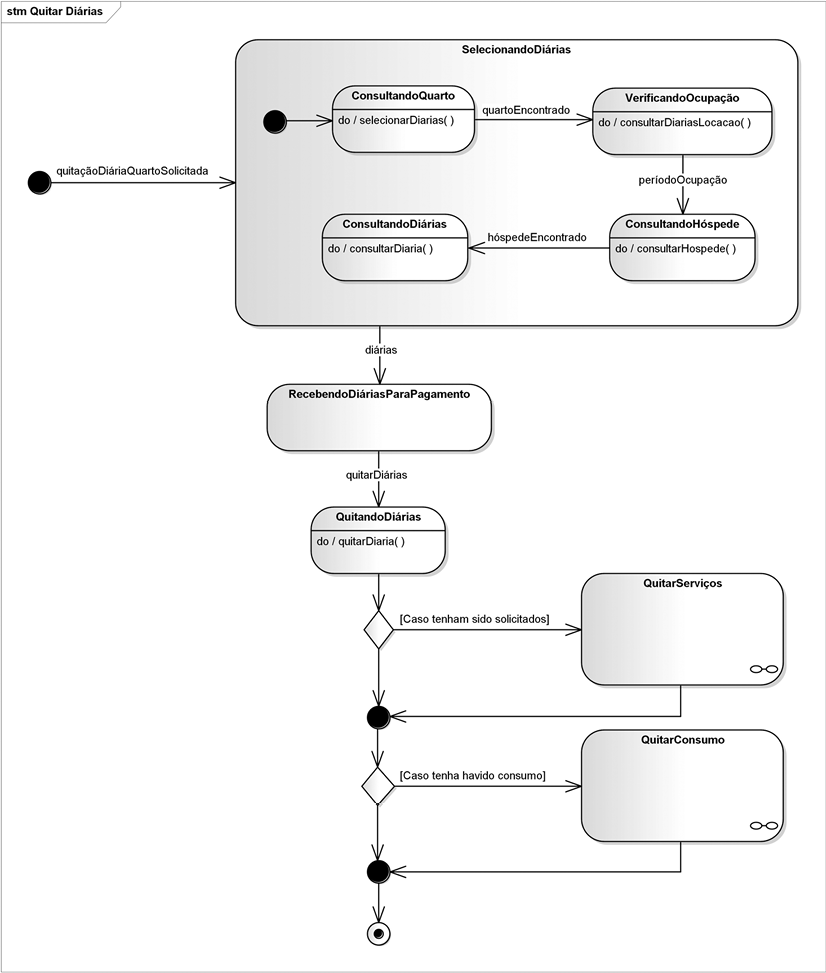
\includegraphics[width=\columnwidth,height=0.55\textheight,keepaspectratio]{imagens/Fig9.28.png}
            \vspace{0.1cm}
            
            {\scriptsize \textbf{Máquina de Estados de Encerramento de Conta (Fig. 9.28 - Guedes)}}
        \end{column}
    \end{columns}
\end{frame}

% =============================================================================
\section{Mapeamento Prático em Python}
% =============================================================================

% -----------------------------------------------------------------------------
% SLIDE 27: Implementando Máquinas de Estado em Código Python
% -----------------------------------------------------------------------------
\begin{frame}[fragile]{Da Modelagem de Estados ao Código Python}
\begin{lstlisting}
class StatusPedido(str, Enum):
    CRIADO = "CRIADO"
    AGUARDANDO_PAGAMENTO = "AGUARDANDO_PAGAMENTO"
    EM_PREPARO = "EM_PREPARO"
    PRONTO_PARA_COLETA = "PRONTO_PARA_COLETA"
    EM_ROTA_DE_ENTREGA = "EM_ROTA_DE_ENTREGA"
    ENTREGUE = "ENTREGUE"
    CANCELADO = "CANCELADO"

class PedidoStateMachine:
    def transitar_para(self, novo: StatusPedido, evento: str, guarda_ok: bool):
        if not guarda_ok:
            raise TransicaoInvalidaException("Condicao de guarda falhou!")
        # 1. Executa acao exit / do estado de origem
        self._executar_exit(self.estado_atual)
        # 2. Transita estado
        self.estado_atual = novo
        # 3. Executa acao entry / do estado de destino
        self._executar_entry(self.estado_atual)
\end{lstlisting}
\end{frame}

% -----------------------------------------------------------------------------
% SLIDE 28: Execução Prática e Rastreamento em Console
% -----------------------------------------------------------------------------
\begin{frame}[fragile]{Executando o Rastreamento de Interação e Estados}
    \begin{columns}
        \begin{column}{0.5\textwidth}
            \textbf{O Script Didático:}
            \begin{itemize}
                \item Arquivo: \texttt{exemplo\_interacao\_estados.py};
                \item Demonstra a execução de checkout com persistência via Repository;
                \item Dispara mensagens síncronas, assíncronas e retornos;
                \item Simula a progressão da máquina de estados com tratamento de exceções de guarda.
            \end{itemize}
        \end{column}
        \begin{column}{0.5\textwidth}
            \begin{exampleblock}{Comando de Execução}
                \scriptsize\texttt{\$ python3 exemplo\_interacao\_estados.py}
            \end{exampleblock}
            \vspace{0.1cm}
            \tiny
            \texttt{[Msg   1.2.1] PedidoService -> GatewayService: debitar(PIX, 70.00)}\\
            \texttt{[Msg 1.2.1.r] GatewayService -> PedidoService: Transacao(APROVADA)}\\
            \texttt{[alt -> Ramo Aprovado] Transicao: AGUARDANDO\_PAGAMENTO -> EM\_PREPARO}\\
            \texttt{[entry / EM\_PREPARO] Notificando painel KDS da cozinha.}
        \end{column}
    \end{columns}
\end{frame}

% =============================================================================
\section{Atividade Prática: TauáDelivery Web}
% =============================================================================

% -----------------------------------------------------------------------------
% SLIDE 29: Contextualização da Atividade Prática
% -----------------------------------------------------------------------------
\begin{frame}{Atividade Prática: TauáDelivery Web (Parte 2, 3 e 4)}
    \begin{columns}
        \begin{column}{0.55\textwidth}
            \textbf{Objetivo do Laboratório:}
            \begin{itemize}
                \item Construir a modelagem comportamental dinâmica completa do caso de uso \textbf{UC03 - Finalizar Pedido e Processar Pagamento}.
            \end{itemize}
            \vspace{0.1cm}
            \textbf{As 4 Etapas da Prática:}
            \begin{enumerate}
                \item \textbf{Parte 1:} Questionário conceitual analítico;
                \item \textbf{Parte 2:} Diagrama de Sequência completo com fragmento \texttt{alt} e repositório;
                \item \textbf{Parte 3:} Diagrama de Comunicação com numeração decimal aninhada;
                \item \textbf{Parte 4:} Diagrama de Máquina de Estados da entidade \texttt{Pedido}.
            \end{enumerate}
        \end{column}
        \begin{column}{0.45\textwidth}
            \begin{block}{Entregáveis}
                Arquivo Markdown com diagramas em Mermaid.js ou PlantUML seguindo a rubrica de avaliação em \texttt{atividade\_pratica.md}.
            \end{block}
        \end{column}
    \end{columns}
\end{frame}

% -----------------------------------------------------------------------------
% SLIDE 30: Exemplo de Apoio 1: Diagrama de Sequência Resolvido
% -----------------------------------------------------------------------------
\begin{frame}{Exemplo Resolvido de Apoio 1: Diagrama de Sequência}
    \centering
    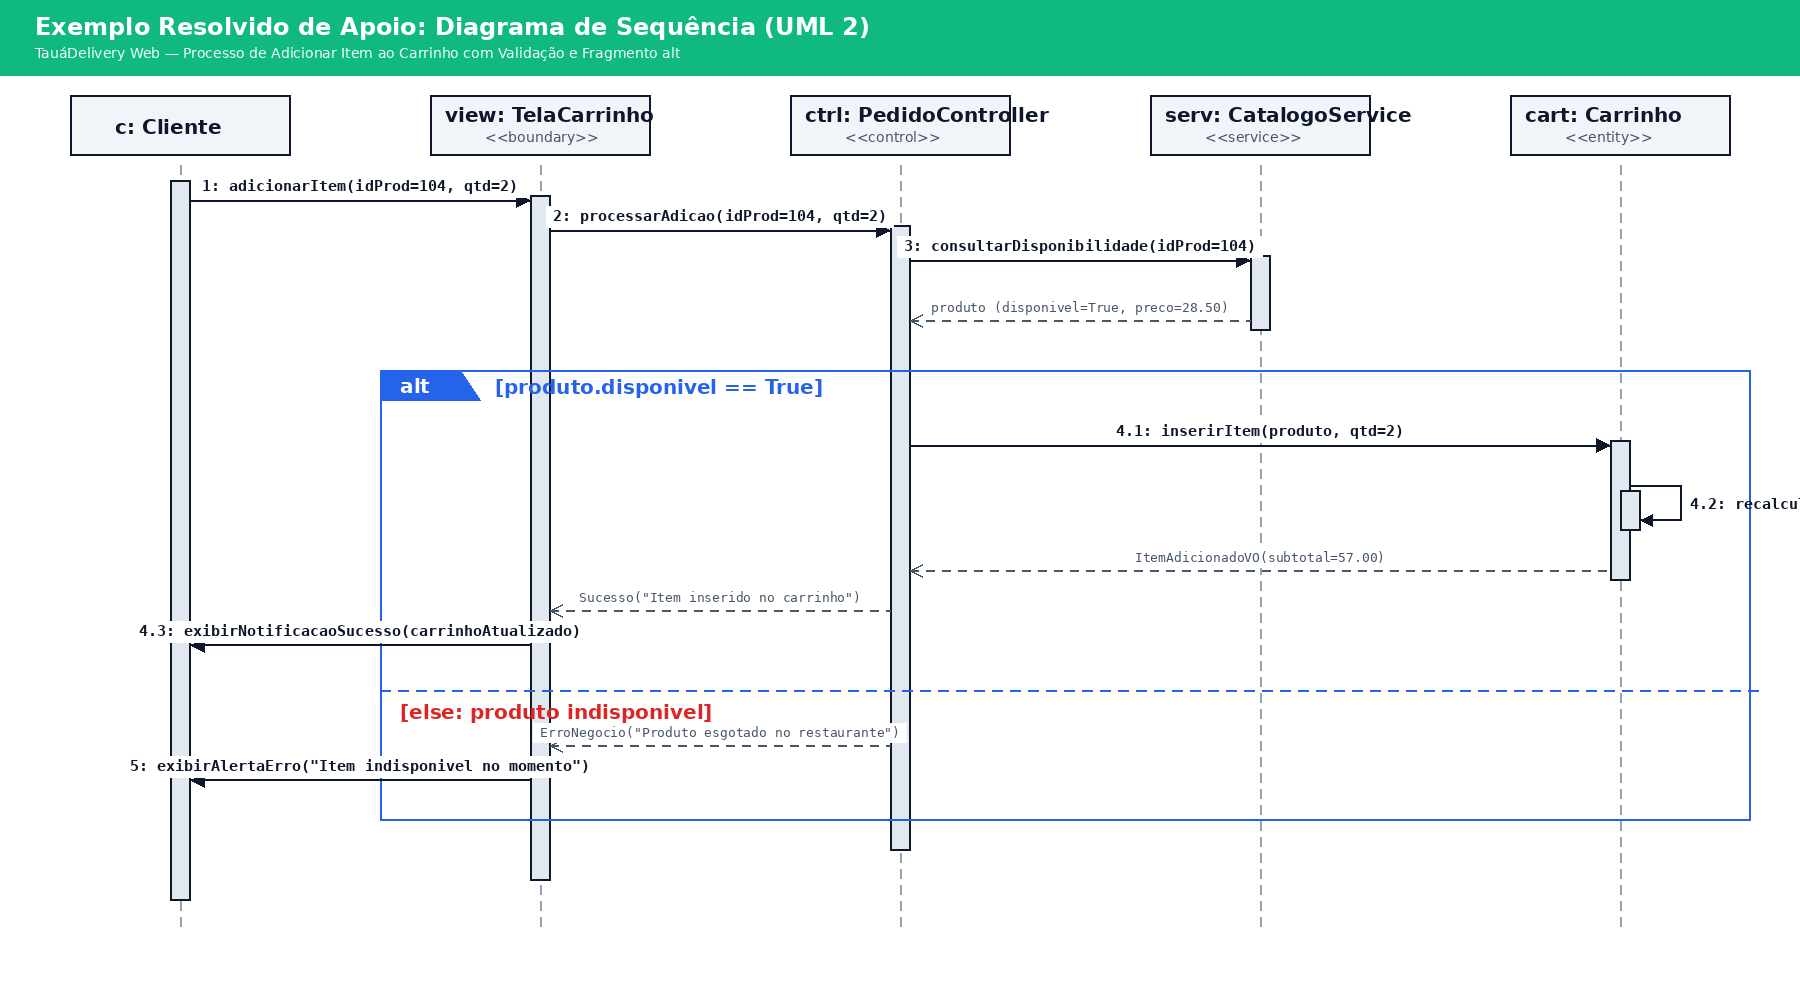
\includegraphics[width=\textwidth,height=0.68\textheight,keepaspectratio]{imagens/modelagem_sequencia_apoio.png}\\[0.05cm]
    {\scriptsize \textbf{Sequência de Adicionar Item ao Carrinho com Validação e Fragmento \texttt{alt}}}
\end{frame}

% -----------------------------------------------------------------------------
% SLIDE 31: Exemplo de Apoio 2: Diagrama de Comunicação Resolvido
% -----------------------------------------------------------------------------
\begin{frame}{Exemplo Resolvido de Apoio 2: Diagrama de Comunicação}
    \centering
    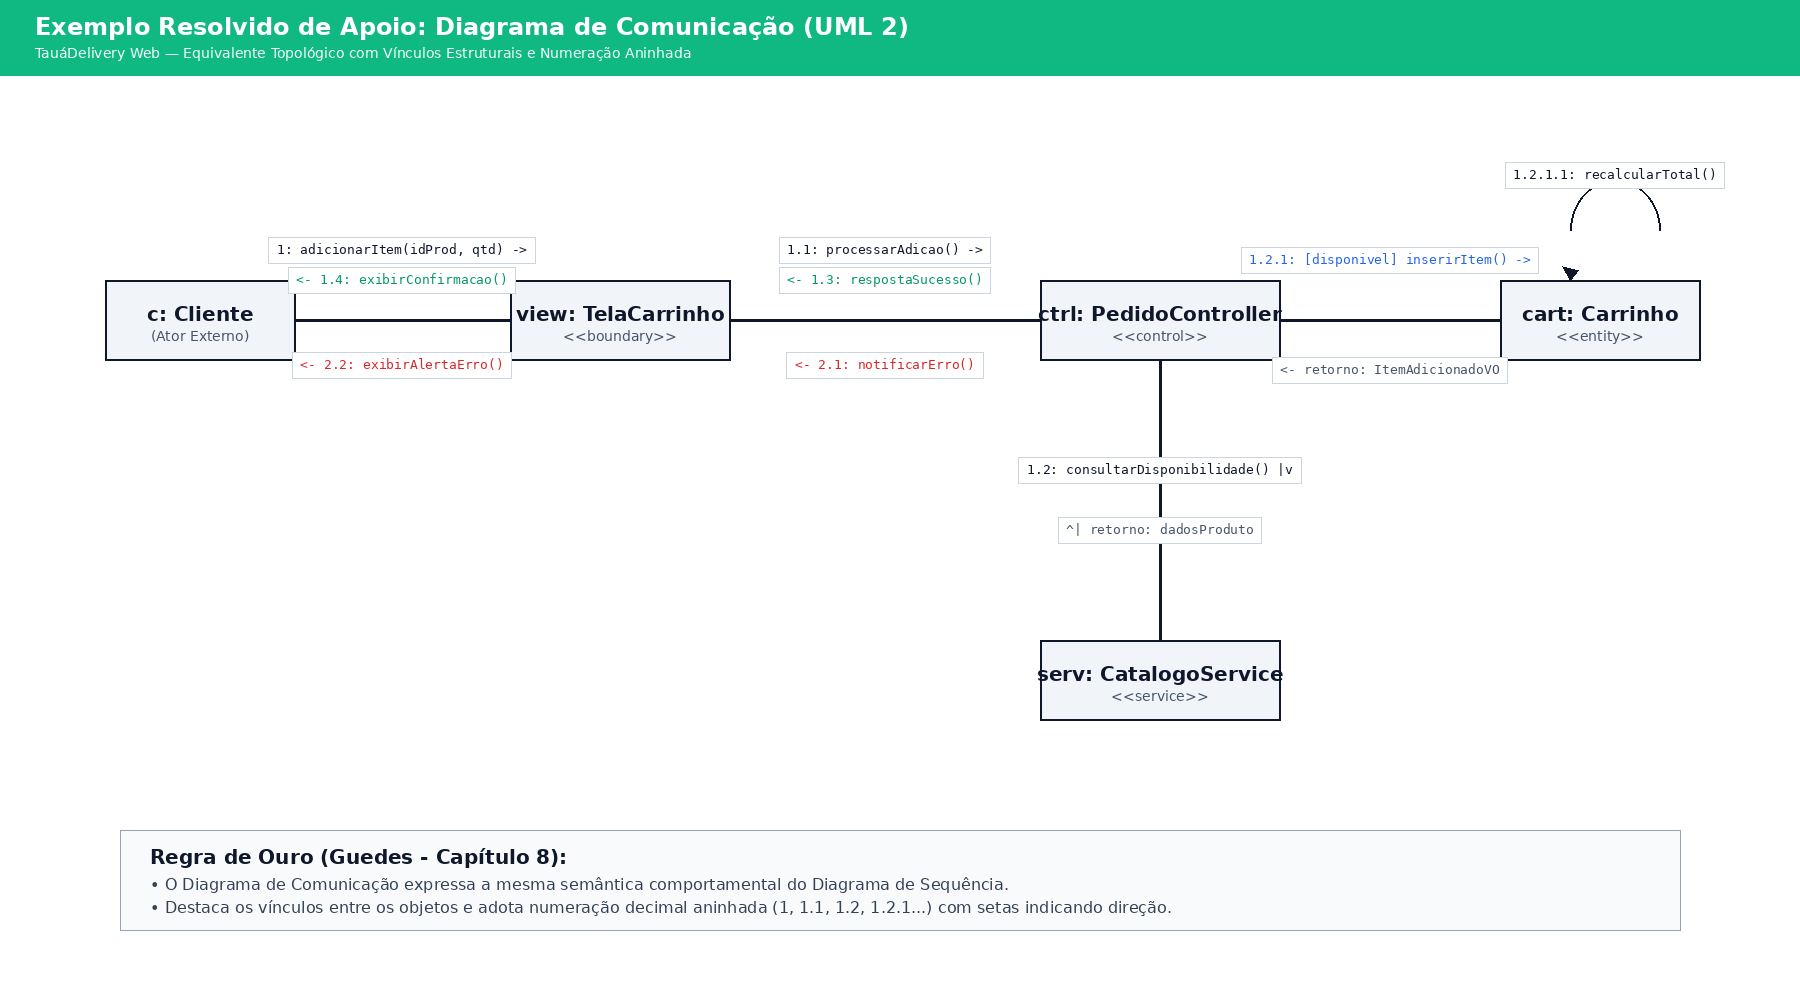
\includegraphics[width=\textwidth,height=0.68\textheight,keepaspectratio]{imagens/modelagem_comunicacao_apoio.png}\\[0.05cm]
    {\scriptsize \textbf{Diagrama de Comunicação correspondente com Vínculos e Numeração Aninhada}}
\end{frame}

% -----------------------------------------------------------------------------
% SLIDE 32: Exemplo de Apoio 3: Máquina de Estados do Pedido Resolvida
% -----------------------------------------------------------------------------
\begin{frame}{Exemplo Resolvido de Apoio 3: Máquina de Estados}
    \centering
    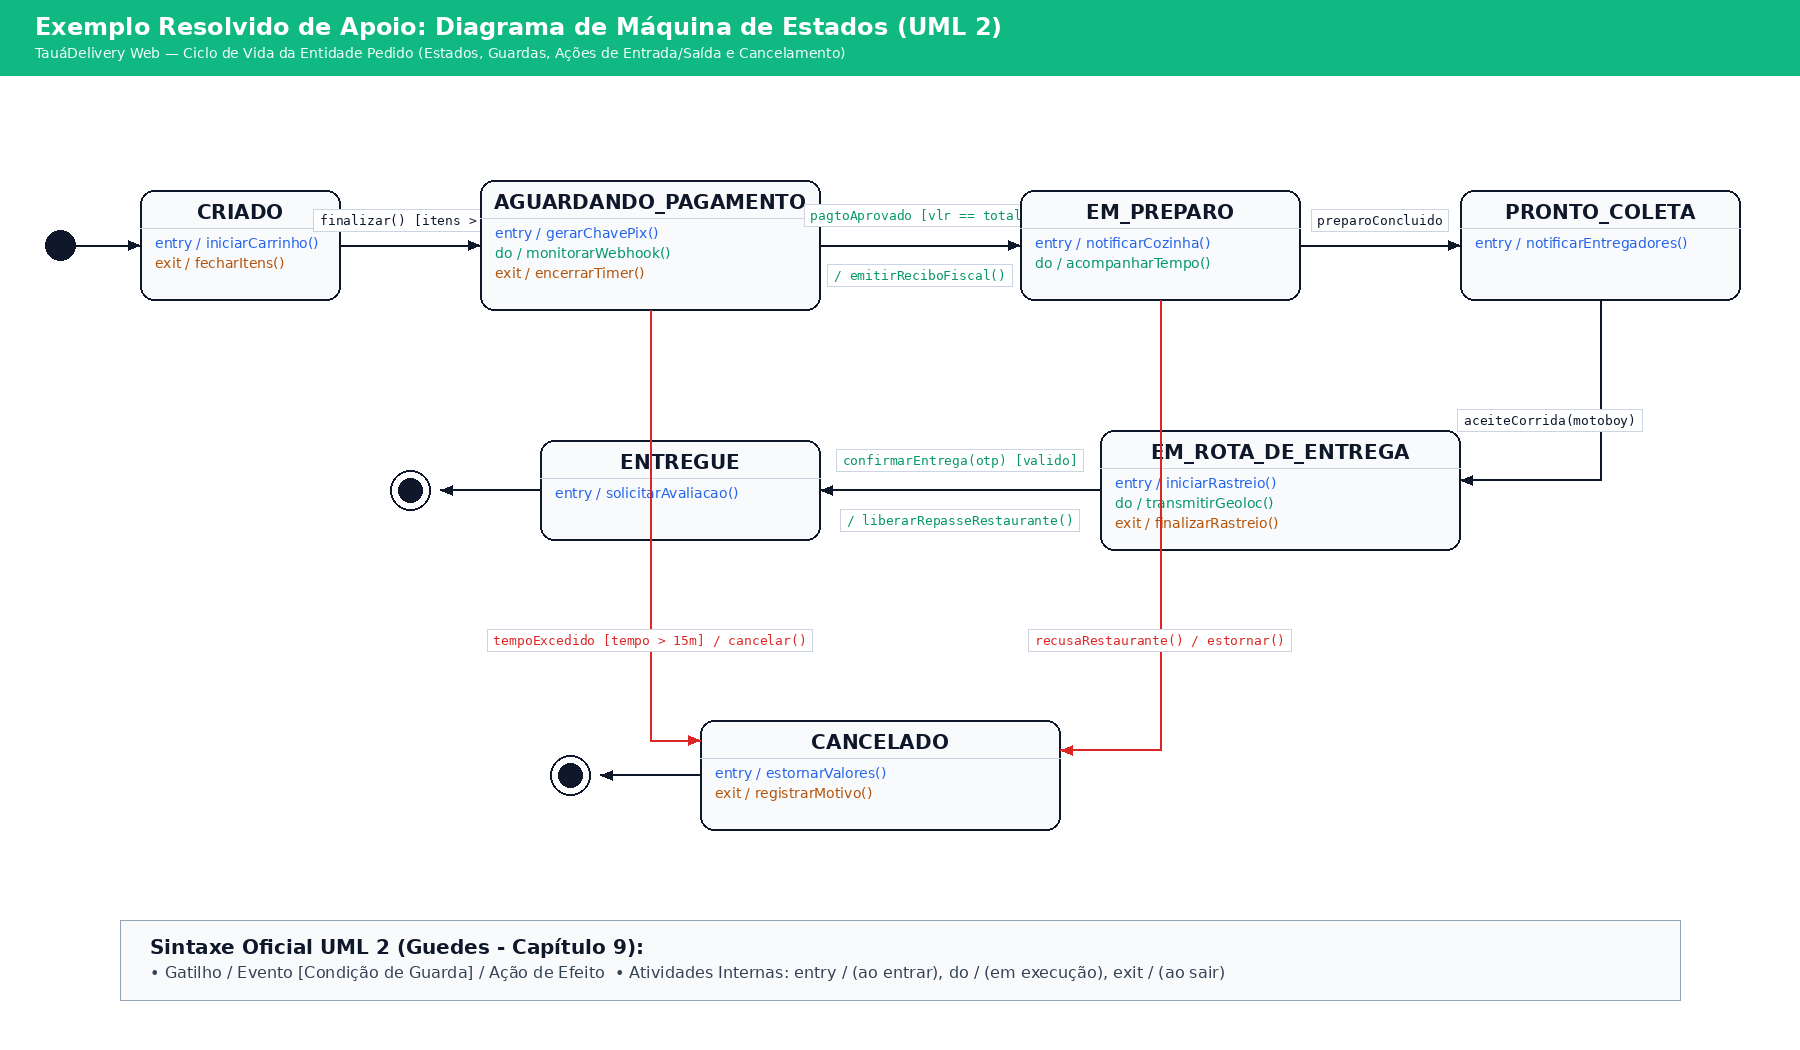
\includegraphics[width=\textwidth,height=0.68\textheight,keepaspectratio]{imagens/modelagem_estados_apoio.png}\\[0.05cm]
    {\scriptsize \textbf{Ciclo de Vida da Entidade Pedido com Guardas e Atividades Internas}}
\end{frame}

% -----------------------------------------------------------------------------
% SLIDE 33: Orientações de Entrega e Critérios de Correção
% -----------------------------------------------------------------------------
\begin{frame}{Orientações de Entrega e Rubrica de Avaliação}
    \begin{columns}
        \begin{column}{0.5\textwidth}
            \textbf{Checklist de Modelagem Obrigatória:}
            \begin{itemize}
                \item As 7 lifelines corretas na Sequência;
                \item Mensagem assíncrona na notificação;
                \item Fragmento \texttt{alt} com ramos aprovado e recusado;
                \item Numeração aninhada estrita na Comunicação;
                \item Todas as atividades \texttt{entry}, \texttt{do} e \texttt{exit} na Máquina de Estados.
            \end{itemize}
        \end{column}
        \begin{column}{0.5\textwidth}
            \begin{block}{Distribuição da Nota (10,0 pontos)}
                \begin{itemize}
                    \item \textbf{Parte 1 (Conceitual):} 2,5 pts
                    \item \textbf{Parte 2 (Sequência):} 2,5 pts
                    \item \textbf{Parte 3 (Comunicação):} 2,5 pts
                    \item \textbf{Parte 4 (Máquina de Estados):} 2,5 pts
                \end{itemize}
            \end{block}
        \end{column}
    \end{columns}
\end{frame}

% =============================================================================
\section{Síntese e Fechamento}
% =============================================================================

% -----------------------------------------------------------------------------
% SLIDE 34: Síntese da Aula e Boas Práticas de Modelagem
% -----------------------------------------------------------------------------
\begin{frame}{Síntese da Aula e Boas Práticas}
    \begin{columns}
        \begin{column}{0.5\textwidth}
            \textbf{Boas Práticas de Interação:}
            \begin{itemize}
                \item Não sobrecarregue um único diagrama de sequência com dezenas de objetos; prefira dividir em subcenários com \texttt{ref};
                \item Sempre explicite se a mensagem é síncrona ou assíncrona;
                \item Utilize o padrão Repository para abstrair consultas complexas.
            \end{itemize}
        \end{column}
        \begin{column}{0.5\textwidth}
            \textbf{Boas Práticas em Máquinas de Estados:}
            \begin{itemize}
                \item Não use máquina de estados para modelar algoritmos ou fluxos procedurais (para isso, use o \textbf{Diagrama de Atividades});
                \item Reserve a máquina de estados para entidades reativas com ciclo de vida significativo (ex.: Pedido, Sessão, Fatura).
            \end{itemize}
        \end{column}
    \end{columns}
\end{frame}

% -----------------------------------------------------------------------------
% SLIDE 35: Conclusão e Próximos Passos (Aula 23)
% -----------------------------------------------------------------------------
\begin{frame}{Conclusão e Próximos Passos}
    \begin{block}{Parabéns pela Conclusão da Aula 22!}
        Agora dominamos a estrutura estática (Classes), o fluxo procedimental (Atividades), a colaboração dinâmica (Sequência e Comunicação) e o ciclo de vida reativo (Máquina de Estados).
    \end{block}
    \vspace{0.2cm}
    \begin{exampleblock}{Próxima Aula (Aula 23)}
        \textbf{Diagramas Arquiteturais da UML 2 (Capítulos 5, 6, 12 e 13 - Guedes):}
        \begin{itemize}
            \item Diagrama de Pacotes e organização em camadas;
            \item Diagrama de Componentes e interfaces fornecidas/requeridas;
            \item Diagrama de Implantação e infraestrutura física/nuvem de servidores.
        \end{itemize}
    \end{exampleblock}
\end{frame}

\end{document}
